%% LyX 2.0.2 created this file.  For more info, see http://www.lyx.org/.
%% Do not edit unless you really know what you are doing.
\documentclass[10pt,a4paper]{article}
\usepackage[utf8]{luainputenc}
\usepackage{graphicx}

%\usepackage{fullpage}
\usepackage{rotating}

\usepackage{listings}\lstset{
        basicstyle=\footnotesize,       % the size of the fonts that are used for the code
        numbers=left,                   % where to put the line-numbers
        numberstyle=\footnotesize,      % the size of the fonts that are used for the line-numbers
        stepnumber=10,                  % the step between two line-numbers. If it's 1, each line 
        breaklines=true,                % Wrap lines that are too long.
        numbersep=5pt,                  % how far the line-numbers are from the code
}

% Title Page
\title{CAP 6616 - Neuroevolution and Generative and Developmental Systems\\Midterm Report}
\author{Anthony Wertz \\ James Schneider}

\begin{document}

\maketitle

\section{Objective}

To evolve a neural network that provides unique transformations of
human faces.

\section{Procedure}

\label{sec:procedure}

Using OpenCV we detect a face in any image and transform the image for input to the neural network. OpenCV is a toolkit for many computer vision tasks which is be used to identify and extract faces from an image. An extracted face is isolated and sent into the deforming network which applies some transformation. An interactive evolutionary process is used in order to generate the transformations used. The evolved neural network scans accepts a normalized (-1 to 1) coordinate, centered at the middle of the images, and returns a resulting coordinate indicating where on the original image pixel data should be pulled from. The evolutionary process takes place within a graphical user interface (GUI) which presents a small population of fifteen images to the user and allows him or her to select any number of preferred transformations. These are the basis for continued evolution.

The neuroevolutionary process is be implemented using the HyperNEAT C++ software as a basis while Python is be used as the main means of processing the results and presenting the options to the user. The two languages interact by providing Python bindings to the HyperNEAT code base. The interaction of the systems is depicted in figure \ref{fig:arch}.

\begin{figure}
    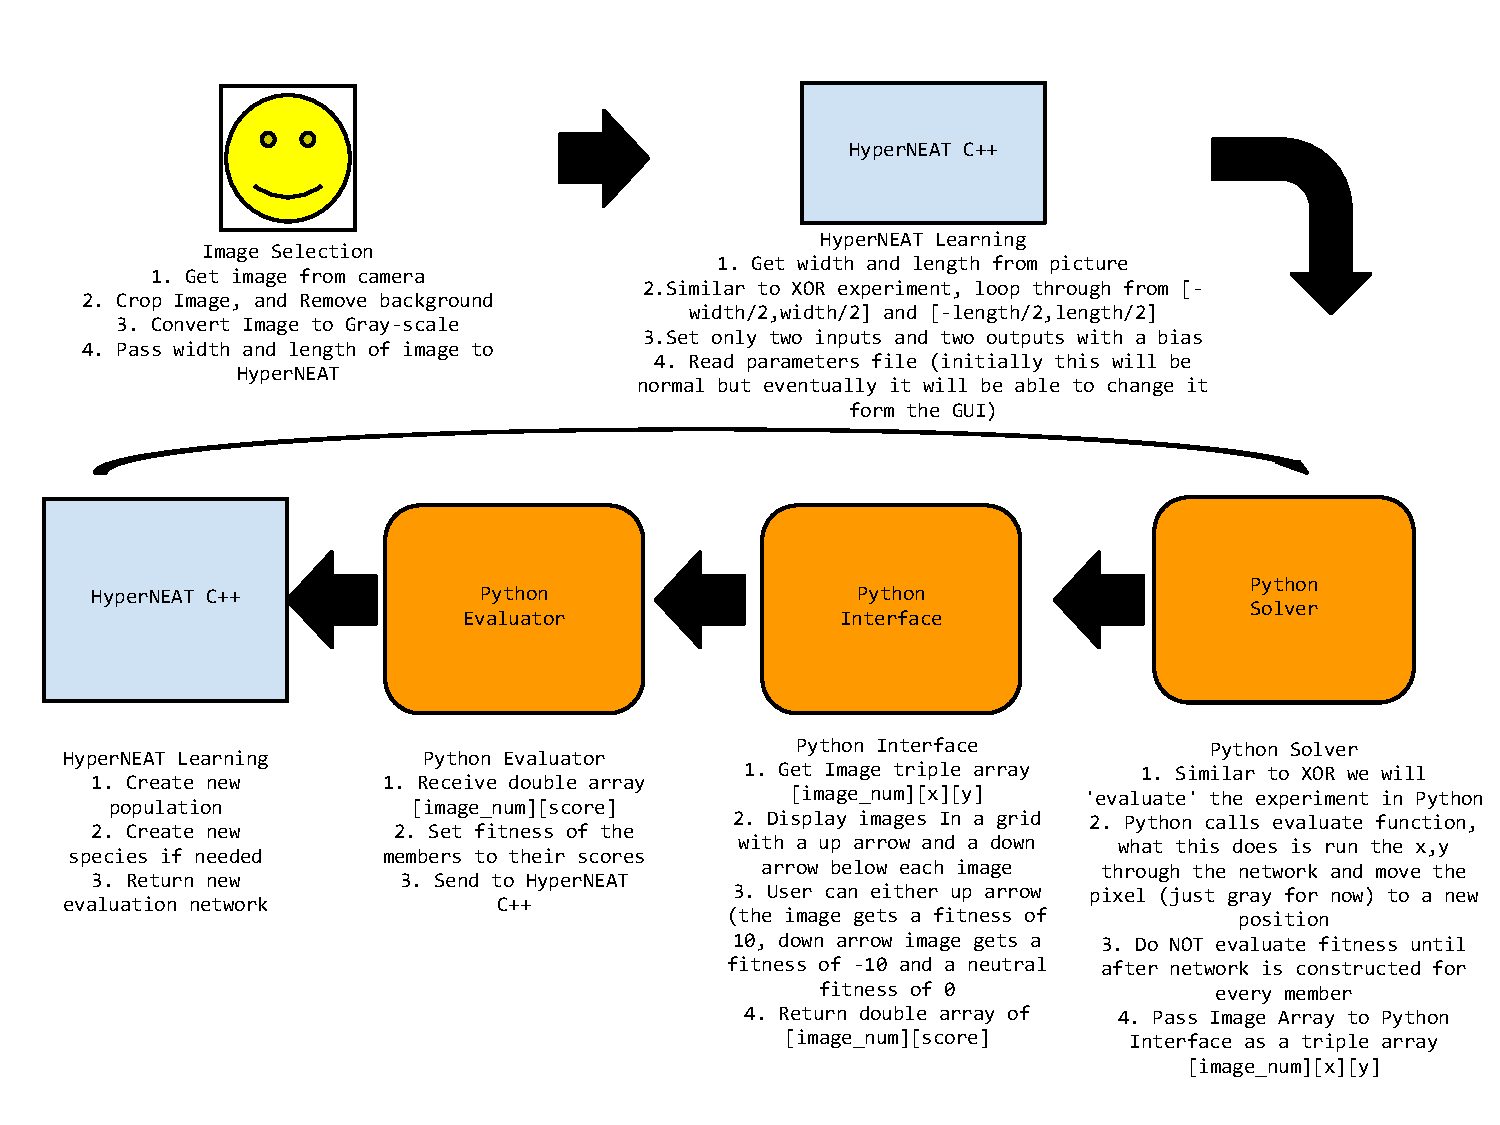
\includegraphics[width=\textwidth]{rec/arch.pdf}
    \caption{Architecture}
    \label{fig:arch}
\end{figure}

As may be seen in figure \ref{fig:arch}, HyperNEAT C++ is be used to manage the internal processing of the main HyperNEAT components as that architecture already exists. However the Python system built is used to display the population (through a GUI built with Qt), evaluate the viability of offspring (e.g. determine the fitness of population individuals via operator input), and send the results back to the HyperNEAT C++ layer for evolution.

The current GUI interface may be seen in figure \ref{fig:gui}. This figure shows the general layout where a user is able to select an input image of a face to view and evolve the deformation networks. A network distortion rasterizer has been built to utilize any given network representing a distortion in normalized coordinates to determine a new image. As shown, the networks represent unique and (sometimes) interesting distortions to the original image. The favored images may then be selected and evolved by clicking ``Evolve'' which prompts the evolution functionality in HyperNEAT.

As shown in the display, evolution parameters are be available to the operator to change on the fly during evolution. This allows adjustment of parameters throughout the process so a unique evolution can occur every time the application is used.

Current progress to this effect includes a large overhaul of the Python bindings available in the original HyperNEAT C++ code distribution to allow for Python tests to be built, the development of a new experiment module within HyperNEAT to support the necessary functionality, and the development of a graphical user interface to allow operator interaction with the evolutionary process. Most of the original work is presented in the source section in \ref{sec:source}, though some minor changes were omitted for brevity in this document.

\section{Questions}

Many questions arose in the work on this project that remain to be answered.

\begin{enumerate}
    \item Can feature extraction and image registration be used to generalize the deformation process across different images and allow deforming of faces at different angles (even if warping to a neutral orientation before deformation is required)?
    \item Will supplying information on the features of the face be useful to the evolution of deformations?
    \item Can image features be used as a means of filtering out redundant transformations and supplying a criteria for a ``novelty search'' in the evolutionary process to supply the operator with unique transformations?
    \item Can and should the network be seeded somehow to promote symmetry in the generated deformations?
    \item Can the deformation process (including face detection, neutralizing, deformation, then rewarping) be completed in real time?
\end{enumerate}

\section{Output}

The GUI provides visual feedback as to the progress of the evolutionary process. It also allows the user to output favored deformations (the image, not the network). The GUI will output the ``best'' networks as well as the entire last generation when the application is exited, but in the future support for exporting specific networks will be added.

As described in section \ref{sec:procedure}, the GUI in figure \ref{fig:gui} is the current operator interface.

\begin{figure}
    \centering
    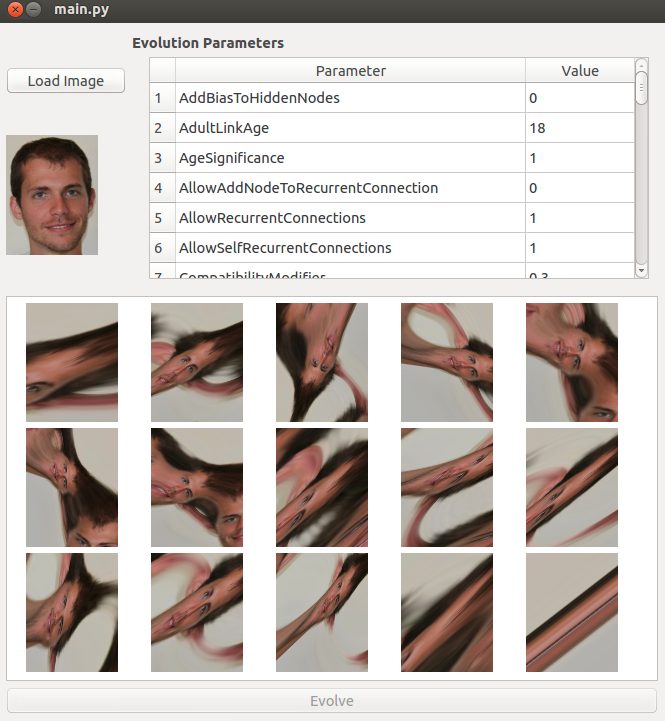
\includegraphics[width=\textwidth]{rec/gui}
    \caption{GUI Prototype}
    \label{fig:gui} 
\end{figure}

\section{Software}

The following is a summary of the major software libraries used in the project:

\begin{enumerate}
    \item HyperNeat v4.0 C++ (along with associated packages: TinyXMLDLL and JG template library
    \item pyQt framework v4.2.8 for the GUI and processing
    \item OpenCV v 2.4
    \item Boost (especially for Python bindings)
\end{enumerate}

\section{Analysis}

\begin{figure}
    \centering
    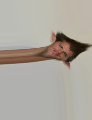
\includegraphics[scale=2]{rec/elfhead.jpg}
    \caption{``Pez elf head'' output}
    \label{fig:common}
\end{figure}


As seen in \ref{fig:gui} the output of the current algorithm is extremely noisy. Presently, the most seen output example can be best described as an elf-like face distortion (pointed ears and chin) and an elongated neck (the dubbed ``elf head Pez dispenser'' transformation, see figure \ref{fig:common}). The CPNN that produces this image is fairly simple for an odd transformation (as seen in figure \ref{fig:CPNN}) consisting of only three hidden nodes that only effect the x-axis. This image is so common amongst the output of the algorithm that we are attempting to determine why the bias toward this very specific deformation exits and analyzing methods to increase diversity within our evolved systems. We have observed the effect that when a user is evolving images the number of generations usually does not extend past 50, due in large part to the user quickly getting tired of picking images individually to evolve and eventually decaying into a pseudo-random type of search. This pseudo-random search makes it such that the CPNN's quickly start to converge on an answer as the species start to mimic each other in their genotype but vary in large ways with the phenotypes. Ideally these phenotype variations would be good, but because most of these phenotypes produce such a big distortion effect they are unlikely to be chosen by the human for evolution and left on the cutting room floor. 

It is obvious what will happen in the situation described above as the slightest change to the genotype has a large impact on the phenotype: eventually those networks with larger variation will be evolved out due to user selection. This promotes a uniformity across the species with the phenotype expressed slightly differently, e.g. rotated along the y-axis as opposed to the x-axis. The uniformity eventually reaches endemic proportions with the all species converging on what that user preferred in initial populations. In this situation the first random population has a large effect on the final image. This represents a fundamental challenge in our evolutionary process that must be rethought for future versions. A novelty search or the use of prior information may be include in the algorithmic process in order to combat this unwanted convergence.

\begin{figure}
    \centering
    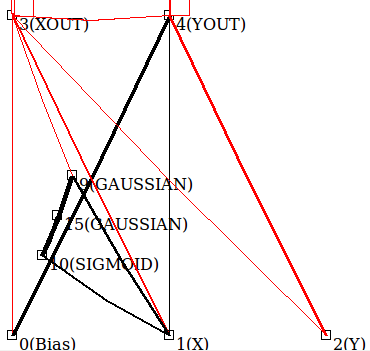
\includegraphics[width=0.5\textwidth]{rec/neuralnet}
    \caption{``Pez elf head'' CPNN }
    \label{fig:CPNN}
\end{figure}

\section{Timeline and Work Distribution}

The following is the timeline and work distribution. Completed tasks are denoted in italics.

\begin{enumerate}
    \item \textit{9/12 - 9/24: Get build environment working between Windows and Ubuntu (hyperNEAT and C++ bindings); use environment to build XOR using python. Work Distribution: Independently get build working on respective platforms; independently implement XOR.}
    \item \textit{9/24 - 9/28: Build initial project architecture modules: (1) the python/hyperNEAT module that evolves CPPNs and sends the result to the user for evolution; (2) python/GUI module that displays the results sent by module 1, allows user selection, and returns the selection back to module 1 for further evolution. Work Distribution: Collaboratively determine python interface between modules; independently build first pass of respective modules; collaboratively work on implementation.}
    \item \textit{9/28 - 10/3: Independently compile necessary documentation and graphics for respective modules; collaboratively compile documentation linking the two and considering the overall system architecture.}
    \item \textit{10/3 - 10/24: Experiment with evolution to attempt to evolve an interesting deformation (independently); through experimentation work out any software bugs; this is the baseline project implementation.}
    \item \textit{10/24 - 10/29: Consolidate interesting findings, issues, and experiences into the midterm report and presentation.}
    \item 10/29 - 11/26: Use time as buffer to finish work on the baseline if good results weren’t obtained. If acceptable results were found, attempt to increase applicability and complexity by looking at extensions including: detecting image features to be used in the transform instead of just pixel locations; integrating evolved neural nets in a video (real time). 
    \item 10/26 - 10/29: Complete Midterm report and Midterm Presentation. 
    \item 10/30 - 11/10: Implement ``Haar Cascades'' to detect facial features. These facial features will be the only ones evolved. The facial features will take the place of the whole image and instead of evolving everything on the image including head position we will just evolve these individual features.
    \item 11/11 - 11/26: Collect images, videos and perform basic statistical analysis on the outputs. Perform a basic user study and develop an outline for the final paper and presentation. Write up analysis about project and discussion sections for final paper.
    \item 11/27 - 12/2: Finish Final presentation and final paper.
    \item 12/2 - 12/7: Complete final paper.
\end{enumerate}

\section{Source Code}

\label{sec:source}

\subsection{PyHyperNEAT.cpp}

\lstinputlisting[language=C++]{../../external/HyperNEAT/NE/HyperNEAT/PyHyperNEAT/src/PyHyperNEAT.cpp}

%\subsection{HCUBE\_ExperimentRun.cpp}
%\lstinputlisting[language=C++]{../external/HyperNEAT/NE/HyperNEAT/HyperCube_NEAT/src/HCUBE_ExperimentRun.cpp}



\subsection{ImageExperiment.h}

\lstinputlisting[language=C++]{../../src/hyperneat/ImageExperiment/ImageExperiment.h}


\subsection{ImageExperiment.cpp}

\lstinputlisting[language=C++]{../../src/hyperneat/ImageExperiment/ImageExperiment.cpp}


\subsection{GUIWindow.py}

\lstinputlisting[language=Python]{../../src/gui/GUIWindow.py}


\subsection{PopulationModel.py}

\lstinputlisting[language=Python]{../../src/gui/PopulationModel.py}
\end{document}
